\chapter{Dasar Desain 3D Model Fusion 360}

\section{Tujuan}
\begin{enumerate}
    \item Belajar mendesain sirkuit elektronik menggunakan software
    \item Mengetahui fungsi setiap komponen dan cara implementasinya
    \item Memahami proses menyusun komponen agar bisa digunakan bersamaan dengan komponen lain
    untuk melakukan fungsi tertentu
    \item Untuk memperkenalkan beberapa konsep dasar dan teknik laboratorium dalam mendesain
    schematic dan PCB
    \item Mendesain rangkaian PCB yang nantinya dapat dicetak menjadi komponen dengan fungsi
    tertentu
\end{enumerate}

\section{Dasar Teori}
Secara sederhana, Enclosure adalah housing logam atau plastik yang dirancang untuk menutupi dan
melindungi disk drive, chip, ataupun board didalamnya dari kerusakan serta risiko lain yang bisa
membahayakan fungsionalitas dan keutuhan komponen didalamnya. Enclosure pada umumnya dapat
menampung satu board, dan memiliki ukuran yang pas dan sesuai, namun tetap memiliki lubang dan celah
sehingga bioard didalamnya masih bisa untuk dihubungkan ke komputer host.

Enclosure case yang efektif memungkinkan untuk ditaruh board dengan tepat, tidak sempit ataupun
longgar, mekanisme penutupan enclosure bisa menggunakan slide, mur, ataupun seperti lego sehingga
tetap tertutup meskipun digoyang dan digerangkan dengan gaya tertentu. Selain itu, enclosure ini
berfungsi untuk melindungi board dari hal-hal seperti kabel dengan tegangan tertentu yang dapat
membuat arus pendek pada board. Berikut referensi desain enclosure

    \begin{figure}[H]
        \centering
        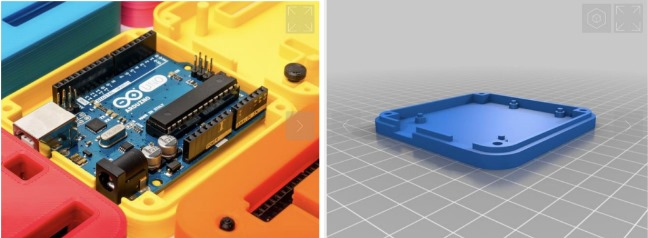
\includegraphics[width=1\linewidth]{P3/img/image1.jpg}
        
    \end{figure}

    \begin{figure}[H]
        \centering
        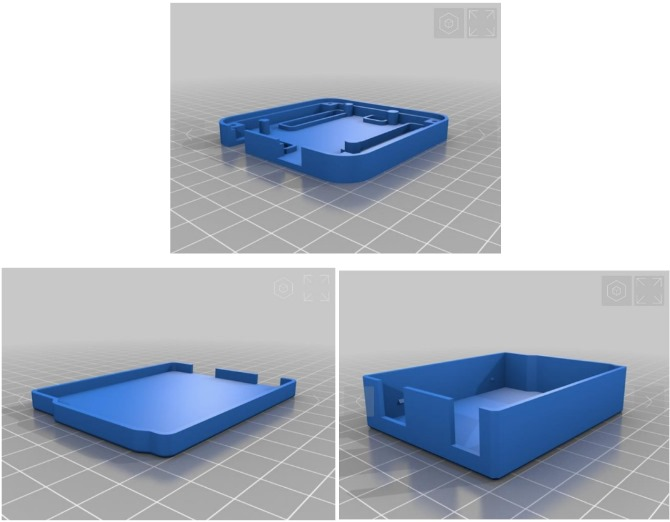
\includegraphics[width=1\linewidth]{P3/img/image2.jpg}
    \end{figure}

Kesalahan yang seringkali dijumpai pada proses desain 3D yaitu alur kerja yang terlalu repetitive ataupun
bertele-tele, karena sebenarnya fitur software banyak yang kurang di-explore sehingga saat
menggunakan software, fitur yang digunakan kurang membantu pengerjaan desain atau bahkan
memperlamanya. Untuk itu hendaknya mencari referensi, dokumentasi, ataupun inspirasi yang terdapat
di sekitar seperti lego, laptop, ataupun projektil lain yang dapat ditiru, amati, dan modifikasi desainnya

\section{Kebutuhan}
\begin{enumerate}
    \item Berdoa kepada Tuhan Yang Maha Esa
    \item PC yang terinstall software Autodesk Fusion 360
    \item File 3D board untuk fitting ke enclosure
\end{enumerate}

\section{Tugas Pendahuluan}
\begin{enumerate}
    \item Baca dan pahami Technical Guide terlebih dahulu!
    \item Baca Panduan Instalasi Autodesk Fusion 360
    \item Baca Panduan Tools Autodesk Fusion 360
\end{enumerate}

\section{Eksperimen 1: Membuat Enclosure PCB}
Buatlah enclosure dari PCB yang disediakan. Enlcosure harus terbagi setidaknya menjadi dua bagian yaitu
\textbf{“Bawah”} sebagai tumpuan PCB dan \textbf{“Atas”} sebagai penutup enclosure. Enclosure juga harus memiliki
lubang power untuk tempat memberi tegangan PCB.

\begin{enumerate}
    \item Sebelum mendesain, upload lah file model 3D dengan type file .stp yang sudah disediakan. Untuk
    mengupload model klik \textbf{“Upload”} di panel sebelah kiri.
        \begin{figure}[H]
            \centering
            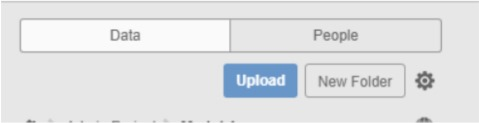
\includegraphics[width=0.5\linewidth]{P3/img/image3.jpg}
        \end{figure}

    \item Untuk memulai mendesain Enclosure klik pada \textbf{“file”} dan klik pada \textbf{“New Design”} atau juga saat
    membuka fusion otomatis new design akan terbuka sendirinya. Setelah new design terbuka klik
    save (ctrl + s) dan beri nama terserah.
        \begin{figure}[H]
            \centering
            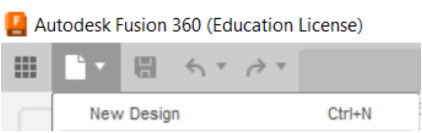
\includegraphics[width=0.5\linewidth]{P3/img/image4.jpg}
        \end{figure}

    \item Langkah selanjutnya adalah memasukan model PCB 3D yang sudah diupload sebelumnya. Untuk
    memasukan model PCB klik kanan pada model tersebut lalu klik \textbf{“Insert into current Design”}.
        \begin{figure}[H]
            \centering
            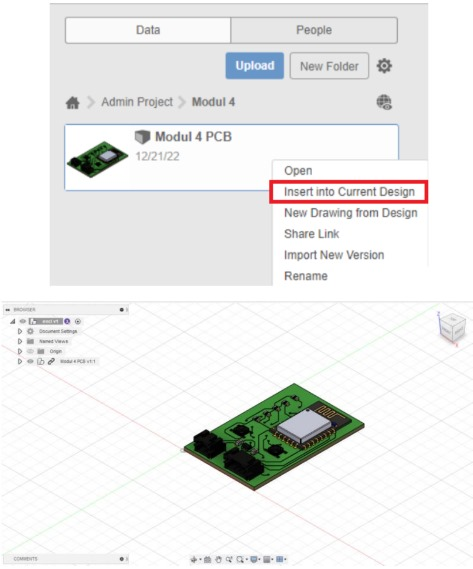
\includegraphics[width=0.5\linewidth]{P3/img/image5.jpg}
        \end{figure}

        \item Saat membuat enclosure terdapat beberapa tools yang tersedia. Berikut beberapa tools yang
        akan sering digunakan dalam pembuatan enclosure:
            \begin{figure}[H]
                \centering
                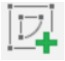
\includegraphics[width=0.1\linewidth]{P3/img/image6.jpg}
            \end{figure}
        \begin{flushleft}
    Sketch: menggambar sketsa 2D dari bentuk yang akan dibuat. Sketsa ini dapat digunakan
    bersama Extrude untuk membuat nya menjadi body 3D.
        \begin{figure}[H]
            \centering
            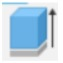
\includegraphics[width=0.1\linewidth]{P3/img/image7.jpg}
        \end{figure}
    Extrude: Mengatur ukuran dari body. Bisa digunakan untuk memperpanjang atau
    memperpendek suatu sisi dari body.
        \begin{figure}[H]
            \centering
            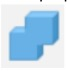
\includegraphics[width=0.1\linewidth]{P3/img/image8.jpg}
        \end{figure}
    Combine: Menggabungkan dua atau lebih body menjadi satu.
        \begin{figure}[H]
            \centering
            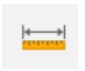
\includegraphics[width=0.1\linewidth]{P3/img/image9.jpg}
        \end{figure}
    Measure: Mengukur body Model 3D
        \begin{figure}[H]
            \centering
            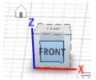
\includegraphics[width=0.1\linewidth]{P3/img/image10.jpg}
        \end{figure}
    Camera: Menggerakan Camera (Dapat juga menggunakan shift+ klik scroll mouse + gerak
    mouse).
    \end{flushleft}
\end{enumerate}

\section{Aturan Pengerjaan:}
\begin{enumerate}
    \item PBC yang dimasukan digunakan sebagai referensi ukuran enclosure yang akan dibuat. Gunakan
    Tools \textbf{“Measure”} untuk mengukur dimensi dari PCB.
    \item Setelah didapat ukuran PCB Gunakan Tools \textbf{“Sketch”} untuk membuat sketsa 2D yang nanti nya
    akan digunakan Tools \textbf{“Extrude”} untuk mengubahnya menjadi body 3D.
    \item Body-body yang terpisah dapat digabungkan menjadi satu menggunakan Tools \textbf{“Combine”}.
    \item Untuk menvigasi dalam ruang 3D dapat digunakan \textbf{“Camera”} untuk melihat dan mebangung
    dari segala sisi/sumbu.
    \item Buatlah setidak nya dua bagian \textbf{“Bawah”} sebagai tumpuan PCB dan \textbf{“Atas”} sebagai penutup
    enclosure.
    \item Buatlah sekreatif mungkin.
\end{enumerate}

\begin{figure}[H]
    \centering
    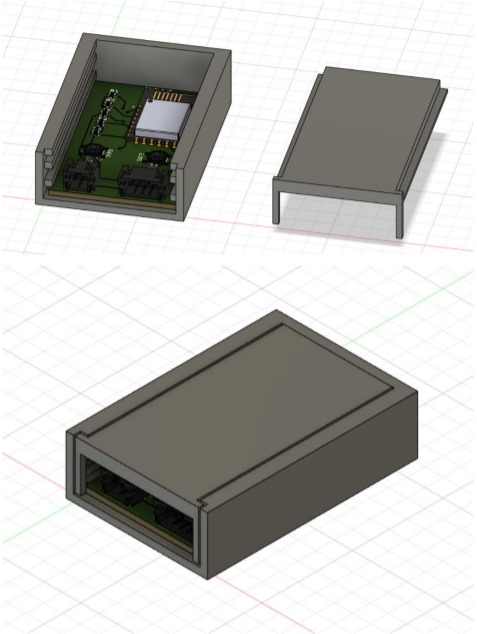
\includegraphics[width=0.6\linewidth]{P3/img/image11.jpg}
\end{figure}